%=====================================================================
% Prototipos corregidos
%   Las tablas y las figuras las genera
%   Prototipos/corregidos/fuente/cambios.py; las imágenes,
%   Prototipos/corregidos/fuente/generar.py. Los originales de
%   Prototipos/ no se modifican.
%=====================================================================
\subsubsection*{Prototipos corregidos}
\addcontentsline{toc}{subsubsection}{Prototipos corregidos}
Las diferencias anteriores, y las que aparecieron al priorizar los casos de uso, se corrigieron en una segunda versión de las pantallas del núcleo, en \texttt{Prototipos/corregidos}. Conservan el estilo de boceto de las originales, que no se modificaron. Tres criterios guiaron las correcciones: mandan los casos de uso; lo que pertenece a un agregado de fase posterior (monedas, cosméticos, amigos, ranking, repeticiones, emotes, espectador) sale de las pantallas del núcleo; y los casos obligatorios que no tenían pantalla la tienen ahora: el registro, el código del segundo factor, la cuenta sin verificar, la activación del segundo factor y la moderación (pantallas \textbf{22a} a \textbf{22h}).

\textbf{Esta segunda versión es anterior al recorte del alcance (\mbox{D-25}).} Las tablas de esta subsección conservan la numeración de casos de uso de entonces, la misma que da la columna \textit{Antes} de los requisitos deseables, y sus justificaciones reflejan la priorización de entonces. Con el alcance actual hay que revisar de nuevo dos grupos de pantallas: las del invitado, los amigos, las invitaciones, el perfil, el ranking y los emotes, que ahora sí entran; y las de moderación manual (\textbf{22e} a \textbf{22h}) y recuperación de contraseña (\textbf{9a}, \textbf{9b}), que ahora son requisitos deseables.

% Archivo generado por Prototipos/corregidos/fuente/cambios.py. No editar a mano.
\begin{center}\small
\begin{longtable}{|L{0.1\textwidth}|L{0.13\textwidth}|L{0.335\textwidth}|L{0.32\textwidth}|}
\hline
\textbf{Pantalla} & \textbf{Casos} & \textbf{Qué cambió} & \textbf{Por qué} \\ \hline
\endfirsthead
\hline
\textbf{Pantalla} & \textbf{Casos} & \textbf{Qué cambió} & \textbf{Por qué} \\ \hline
\endhead
\textbf{3b} Menú principal & \mbox{CU-01}, \mbox{CU-17}, \mbox{CU-18}, \mbox{CU-19} & Se quitan tienda, personalizar, ranking, historial, amigos, el chat global, las monedas y la racha. & Son agregados de fase posterior (\mbox{CU-12} a \mbox{CU-16}, \mbox{CU-29} a \mbox{CU-41}). \\ \cline{3-4}
 &  & Quedan buscar partida, crear sala privada y unirse con código, más ajustes. & Son los casos Must de partida en línea. \\ \cline{3-4}
 &  & Se añade ``cómo jugar'' y un acceso a moderación visible solo para ese rol. & El tutorial es fase posterior; las reglas en texto bastan. La moderación (\mbox{CU-43}) no tenía entrada. \\ \hline
\textbf{6c} Inicio de sesión & \mbox{CU-01}, \mbox{CU-02}, \mbox{CU-03} & Se añaden los campos de nickname o correo y contraseña, y el enlace para recuperar la contraseña. & Diferencia registrada: la pantalla no tenía campos (\mbox{CU-01}). \\ \cline{3-4}
 &  & Se quita ``jugar como invitado''. & \mbox{CU-06} es fase posterior y esquivaría el segundo factor. \\ \cline{3-4}
 &  & Se añade el selector de idioma y el aviso del segundo factor. & \mbox{CU-05} \mbox{RN-03} y \mbox{CON-08}. \\ \hline
\textbf{22a} Registro (nueva) & \mbox{CU-02} & Pantalla nueva: nickname de 3 a 30, correo, contraseña con su regla, fecha de nacimiento (mínimo 8 años), idioma y términos. & El formulario de registro no estaba prototipado (diferencia registrada); campos de \mbox{CU-02} \mbox{RN-01} a \mbox{RN-05} y \mbox{D-06}. \\ \hline
\textbf{22b} Código de segundo factor (nueva) & \mbox{CU-01} & Pantalla nueva: código de 6 dígitos, tiempo restante, intentos, reenviar y cancelar. & GUI\_SecondFactor de \mbox{CU-01} (\mbox{RN-09}: 5 minutos, 3 intentos). Es la restricción \mbox{CON-08} del profesor y no tenía prototipo. \\ \hline
\textbf{22c} Cuenta pendiente de verificar (nueva) & \mbox{CU-01}, \mbox{CU-04} & Pantalla nueva: aviso de correo enviado, reenviar con espera y entrar. & GUI\_PendingVerification de \mbox{CU-01}; sin verificar no se entra (Matriz 2). \\ \hline
\textbf{22d} Activar el segundo factor (nueva) & \mbox{CU-09} & Diálogo nuevo: contraseña actual y código de prueba para activar el segundo factor. & \mbox{CU-09} \mbox{FA-10}; el segundo factor lo exige el profesor y no había dónde activarlo. \\ \hline
\textbf{1f} Buscando rival & \mbox{CU-17} & Se quita el botón ``ampliar rango''; se explica que la ventana de elo se amplía sola. & \mbox{CU-17} \mbox{RN-03}: la ampliación es automática. \\ \cline{3-4}
 &  & Se muestra el reloj elegido. & El modo y el reloj definen la cola. \\ \hline
\textbf{1h} Partida privada: crear o unirse & \mbox{CU-18}, \mbox{CU-19} & El código pasa a seis caracteres sin 0, O, 1 ni I (K7MTQ3). & \mbox{CU-18} \mbox{RN-01}; el prototipo usaba K4M-92. \\ \cline{3-4}
 &  & El código aparece al crear la sala; muros de 1 a 20 y aviso de que no da elo. & \mbox{CU-18} \mbox{RN-04} y \mbox{D-16}. \\ \hline
\textbf{5d} Sala de espera, 2 jugadores & \mbox{CU-18}, \mbox{CU-19} & Se quita ``invitar amigo''. & \mbox{CU-32} es fase posterior. \\ \cline{3-4}
 &  & Código de seis caracteres; ``salir'' avisa que cierra la sala; ``empezar'' inactivo mientras falten listos. & \mbox{CU-18} \mbox{RN-01}, \mbox{RN-07} y \mbox{CU-19} \mbox{RN-03}. \\ \hline
\textbf{5e} Sala de espera, 4 plazas & \mbox{CU-18}, \mbox{CU-19}, \mbox{CU-28} & Se quitan ``eligiendo peón'' y ``abrir a público''. & Los cosméticos son fase posterior y ningún caso abre una sala al público. \\ \cline{3-4}
 &  & El chat de la sala avisa que se filtra y se puede reportar. & Moderación de chat (\mbox{CON-09}, \mbox{CU-28}). \\ \hline
\textbf{19d} Menú de partida & \mbox{CU-22}, \mbox{CU-23} & Se quita ``emotes''. & \mbox{CU-29} es fase posterior. \\ \cline{3-4}
 &  & ``Ofrecer tablas'' dice una vez cada cinco jugadas propias y solo en partidas de dos; se quita ``desde la jugada 10''. & Diferencia registrada; \mbox{CU-22} \mbox{RN-03} y \mbox{D-14}. \\ \hline
\textbf{2g} Fin de partida & \mbox{CU-25} & Se quitan las monedas, la racha, ``ver repetición'' y ``revancha''. & Monedas, rachas y repeticiones son fase posterior; la revancha no está en ningún caso. \\ \cline{3-4}
 &  & Quedan el resultado, la forma de término, el cambio de elo, ``buscar otra'', ``volver al menú'' y ``reportar''. & \mbox{CU-25} pasos 17 a 20 del núcleo y \mbox{CU-42}. \\ \hline
\textbf{6f} Rival desconectado & \mbox{CU-24}, \mbox{CU-26} & ``Reclamar victoria'' queda inactivo con la cuenta atrás hasta los sesenta segundos. & \mbox{D-15} y \mbox{CU-24} \mbox{RN-06}: el rival puede reclamarla solo a los 60 s. \\ \hline
\textbf{20c} Chat en partida & \mbox{CU-28}, \mbox{CU-33}, \mbox{CU-42} & Se quitan las pestañas global y amigos, y el aviso de espectador. & Canales y espectador de fase posterior. \\ \cline{3-4}
 &  & Se añade el aviso de mensaje filtrado y el acceso a silenciar, bloquear y reportar. & \mbox{CU-28} \mbox{RN-02}, \mbox{CU-33} y \mbox{CU-42}. \\ \hline
\textbf{10a} Menú de un jugador & \mbox{CU-33}, \mbox{CU-42} & Se quitan ver perfil, retar, añadir amigo y ver su partida. & Perfil, amigos y espectador son fase posterior. \\ \cline{3-4}
 &  & Quedan silenciar, bloquear y reportar. & Moderación del núcleo. ``Eliminar amigo'' (\mbox{CU-49}) se añadirá con los amigos. \\ \hline
\textbf{10b} Reportar & \mbox{CU-42} & Los motivos pasan a los cinco del dominio: lenguaje ofensivo, acoso, nombre inapropiado, trampas y juego antideportivo. & \mbox{CU-42} \mbox{RN-08} y \mbox{D-23}; el prototipo tenía ``abandono repetido'' y ``otro'' y no tenía acoso. \\ \cline{3-4}
 &  & Se adjuntan las jugadas y el chat de la partida por referencia; se quita la repetición y los enlaces del perfil. & \mbox{CU-42} \mbox{RN-01}; repeticiones y enlaces son fase posterior. \\ \hline
\textbf{10c} Silenciados y bloqueados & \mbox{CU-33} & La explicación dice que el bloqueo impide compartir sala en lugar de invitar. & Las invitaciones son fase posterior (\mbox{CU-32}). \\ \hline
\textbf{10d} Chat restringido & \mbox{CU-28}, \mbox{CU-44} & La restricción se muestra sobre el chat de la partida; se quitan las pestañas global y amigos y la mención a los emotes. & Canales y emotes de fase posterior. \\ \hline
\textbf{9a} Recuperar contraseña: pedir el código & \mbox{CU-03} & Se envía un código de 6 dígitos, no un enlace; se añade el aviso de que la respuesta es la misma exista o no la cuenta y el límite de 5 minutos. & \mbox{CU-03} \mbox{RN-01}, \mbox{RN-04} y \mbox{RN-06}. \\ \cline{3-4}
 &  & Se quita el recuadro del invitado. & \mbox{CU-06} es fase posterior. \\ \hline
\textbf{9b} Recuperar contraseña: código y nueva contraseña & \mbox{CU-03} & Se añade el campo del código con su vigencia y sus 3 intentos, y la confirmación de la contraseña. & \mbox{CU-03} \mbox{RN-04} y \mbox{RN-09}. \\ \hline
\textbf{9f} Ajustes de cuenta & \mbox{CU-05}, \mbox{CU-09}, \mbox{CU-10} & Se añade el segundo factor con su estado. & \mbox{CU-09} \mbox{FA-10} y \mbox{CON-08}. \\ \cline{3-4}
 &  & Se quitan código de amigo, descargar mis datos y borrar cuenta. & Amigos y baja son fase posterior; descargar datos se retiró del alcance (diferencia registrada). \\ \hline
\textbf{12c} Ajustes: idioma & \mbox{CU-12} (solo idioma) & Solo quedan español (México) e inglés. & \mbox{D-21}: los idiomas admitidos son es-MX y en; el prototipo ofrecía portugués, francés, alemán y catalán. \\ \hline
\textbf{7e} Errores de cuenta & \mbox{CU-01}, \mbox{CU-02} & El nickname admite de 3 a 30 caracteres; el bloqueo es de 5, 30 y 60 minutos. & Diferencia registrada; \mbox{CU-01} \mbox{RN-03} y \mbox{CU-02} \mbox{RN-01}. \\ \cline{3-4}
 &  & Se quitan los errores de monedas, skins y amigos; se añaden los de cuenta sin activar, código incorrecto o vencido y edad mínima. & Agregados fuera; errores de \mbox{CU-01}, \mbox{CU-02} y \mbox{CU-04}. \\ \hline
\textbf{7d} Errores de salas y emparejamiento & \mbox{CU-17}, \mbox{CU-19} & El código de ejemplo y el mensaje de formato pasan a seis caracteres sin 0, O, 1 ni I. & Diferencia registrada; \mbox{CU-18} \mbox{RN-01}. \\ \cline{3-4}
 &  & ``Prueba a ampliar el rango'' pasa a ``ampliamos el rango mientras esperas''. & \mbox{CU-17} \mbox{RN-03}. \\ \hline
\textbf{22e} Cola de moderación (nueva) & \mbox{CU-43} & Pantalla nueva: reportes y apelaciones pendientes, con motivo, reportado, reportes que acumula, antigüedad y estado. & GUI\_ModerationQueue; la moderación es obligatoria y no tenía prototipo. \\ \hline
\textbf{22f} Revisar un reporte (nueva) & \mbox{CU-43} & Pantalla nueva: descripción, chat con el reportado resaltado, jugadas, sanciones previas, nota obligatoria y las tres salidas. & GUI\_ReportReview de \mbox{CU-43} (\mbox{RN-07}: nota obligatoria). \\ \hline
\textbf{22g} Aplicar una sanción (nueva) & \mbox{CU-44} & Pantalla nueva: ámbito, tipo, duración, motivo y confirmación en una frase. & GUI\_ApplySanction de \mbox{CU-44} (\mbox{RN-03}, \mbox{RN-06} y \mbox{RN-08}) y \mbox{D-05}. \\ \hline
\textbf{22h} Agregar un moderador (nueva) & \mbox{CU-46}, \mbox{CU-47} & Pantalla nueva: buscar la cuenta, requisitos, motivo obligatorio y la lista de moderadores con ``retirar rol''. & GUI\_AdminPanel de \mbox{CU-46} (\mbox{RN-02}, \mbox{RN-05}) y \mbox{CU-47}. \\ \hline
\end{longtable}
\end{center}


\textbf{Pantallas que no se corrigieron.} Las de casos de fase posterior se corregirán cuando se retomen; la tabla dice qué les falta. Las del núcleo que ya coinciden con los casos se usan tal como están.

% Archivo generado por cambios.py. No editar a mano.
\begin{center}\small
\begin{longtable}{|L{0.16\textwidth}|L{0.25\textwidth}|L{0.49\textwidth}|}
\hline
\textbf{Pantalla} & \textbf{Qué muestra} & \textbf{Por qué no se corrigió} \\ \hline
\endfirsthead
\hline
\textbf{Pantalla} & \textbf{Qué muestra} & \textbf{Por qué no se corrigió} \\ \hline
\endhead
6d & Primera vez: nombre, peón e icono & \mbox{CU-08} es fase posterior. Al retomarla, quitar el campo del nombre (\mbox{D-13}). \\ \hline
9e & Invitado: vincular cuenta & \mbox{CU-07} es fase posterior. Al retomarla, pedir también nickname definitivo y fecha de nacimiento. \\ \hline
2c, 16c & Ranking y evolución del elo & \mbox{CU-35} y \mbox{CU-15} son fase posterior. Al retomarlas, quitar las temporadas. \\ \hline
18f & Errores de modos, IA y búsqueda & La IA y los perfiles son fase posterior. Al retomarla, quitar el límite de cinco sugerencias y los perfiles privados. \\ \hline
16a, 1g, 20a, 21a, 6e, 8e, 10e & Elegir modo, VS, partida, muro, reconexión, cuatro jugadores y aviso de sanción & Ya coinciden con los casos del núcleo: se usan tal como están. \\ \hline
\end{longtable}
\end{center}


% Archivo generado por cambios.py. No editar a mano.
\par\medskip\noindent
\begin{minipage}[t]{0.48\textwidth}
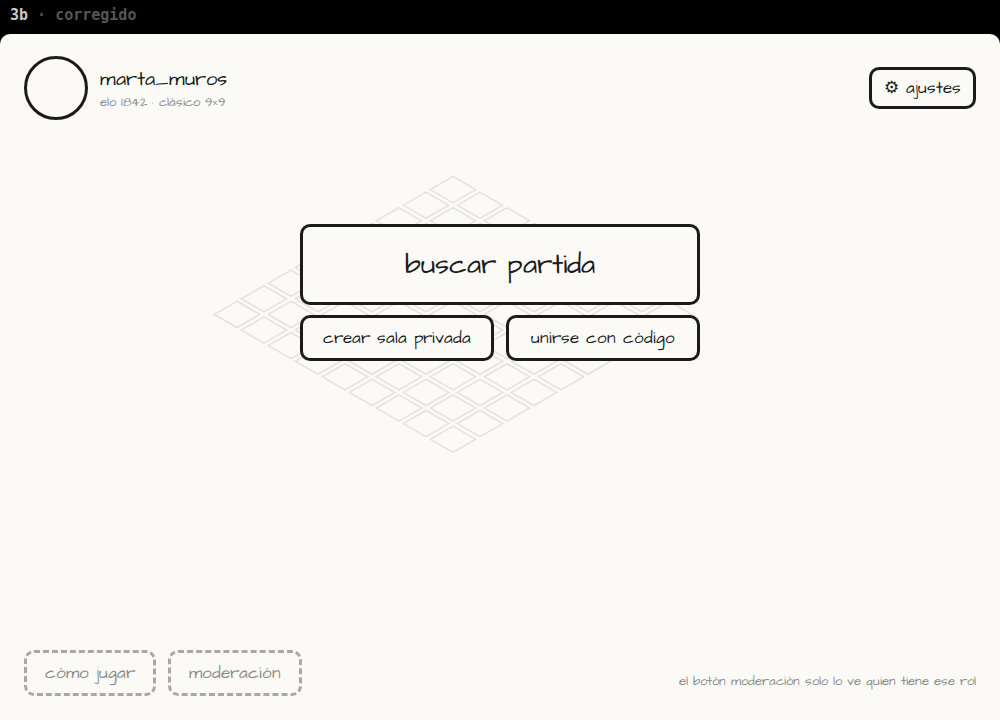
\includegraphics[width=\linewidth]{Prototipos/corregidos/3b}\par\smallskip
{\footnotesize\RaggedRight \textbf{3b corregido: Menú principal}\par}
\end{minipage}\hfill
\begin{minipage}[t]{0.48\textwidth}
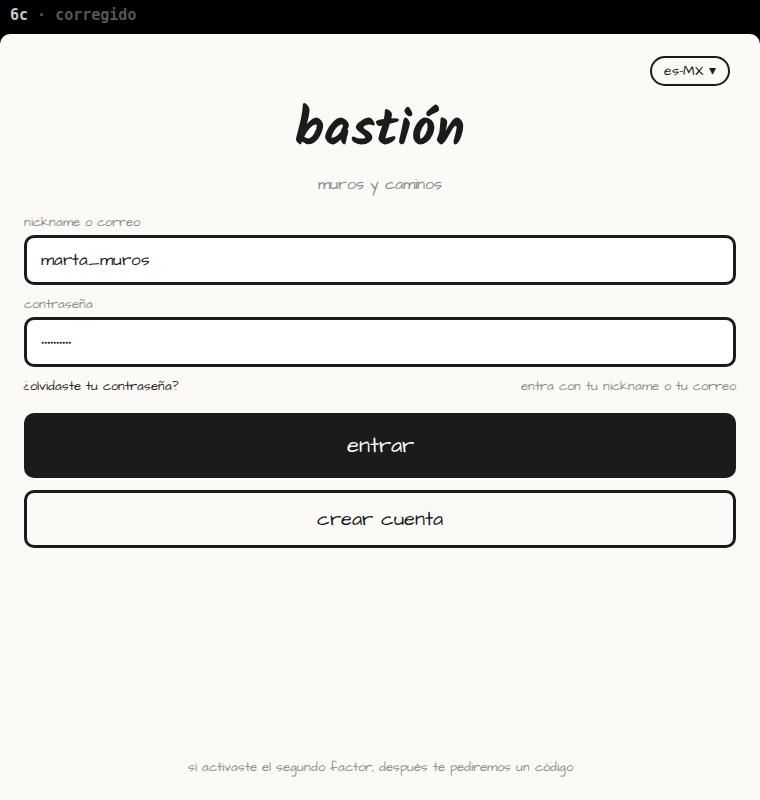
\includegraphics[width=\linewidth]{Prototipos/corregidos/6c}\par\smallskip
{\footnotesize\RaggedRight \textbf{6c corregido: Inicio de sesión}\par}
\end{minipage}
\par
\par\medskip\noindent
\begin{minipage}[t]{0.48\textwidth}
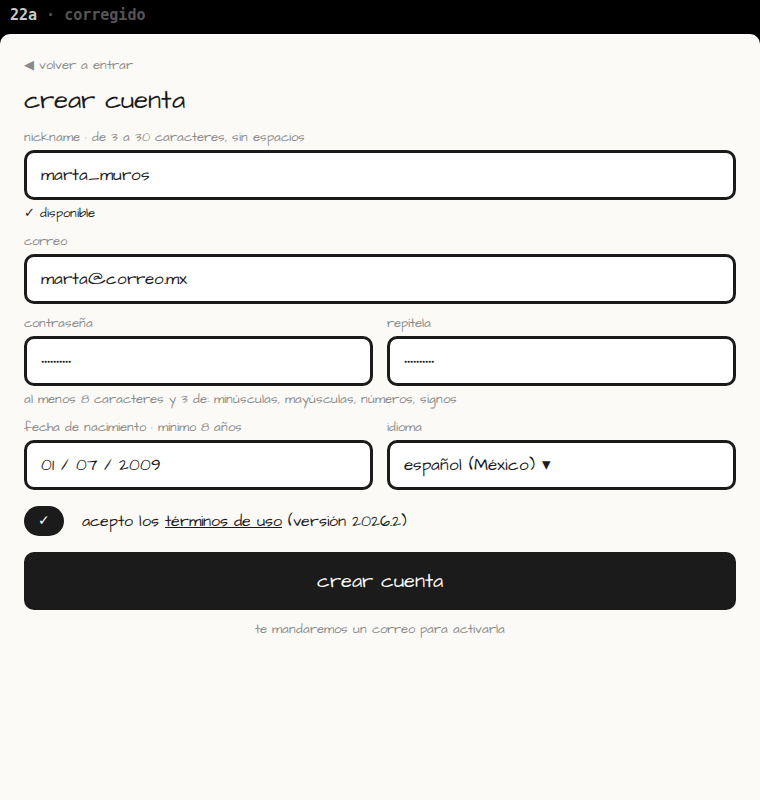
\includegraphics[width=\linewidth]{Prototipos/corregidos/22a}\par\smallskip
{\footnotesize\RaggedRight \textbf{22a corregido: Registro (nueva)}\par}
\end{minipage}\hfill
\begin{minipage}[t]{0.48\textwidth}
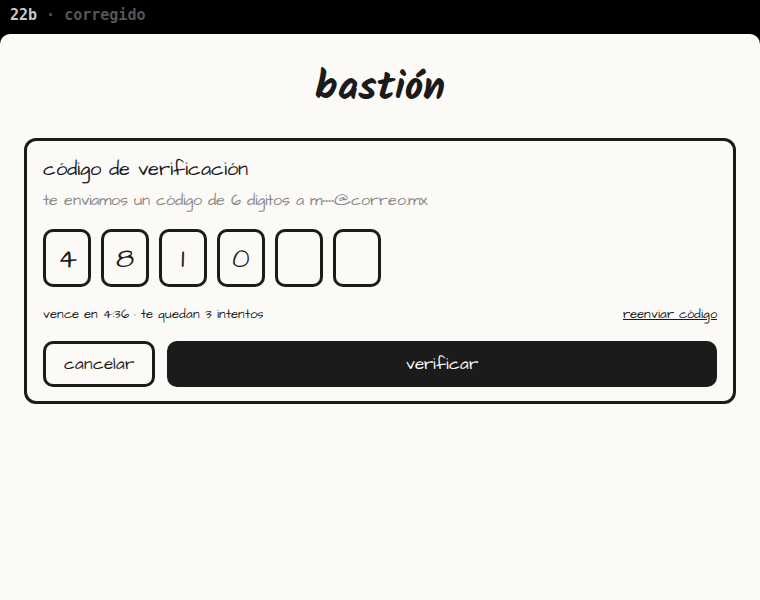
\includegraphics[width=\linewidth]{Prototipos/corregidos/22b}\par\smallskip
{\footnotesize\RaggedRight \textbf{22b corregido: Código de segundo factor (nueva)}\par}
\end{minipage}
\par
\par\medskip\noindent
\begin{minipage}[t]{0.48\textwidth}
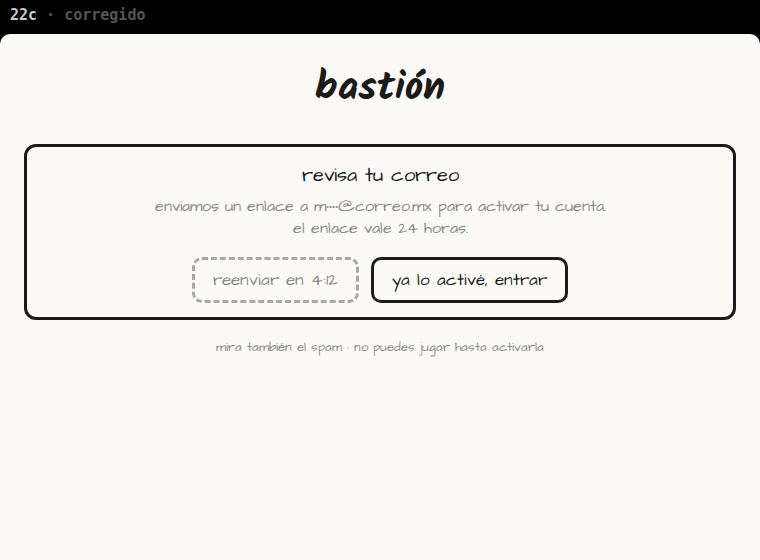
\includegraphics[width=\linewidth]{Prototipos/corregidos/22c}\par\smallskip
{\footnotesize\RaggedRight \textbf{22c corregido: Cuenta pendiente de verificar (nueva)}\par}
\end{minipage}\hfill
\begin{minipage}[t]{0.48\textwidth}
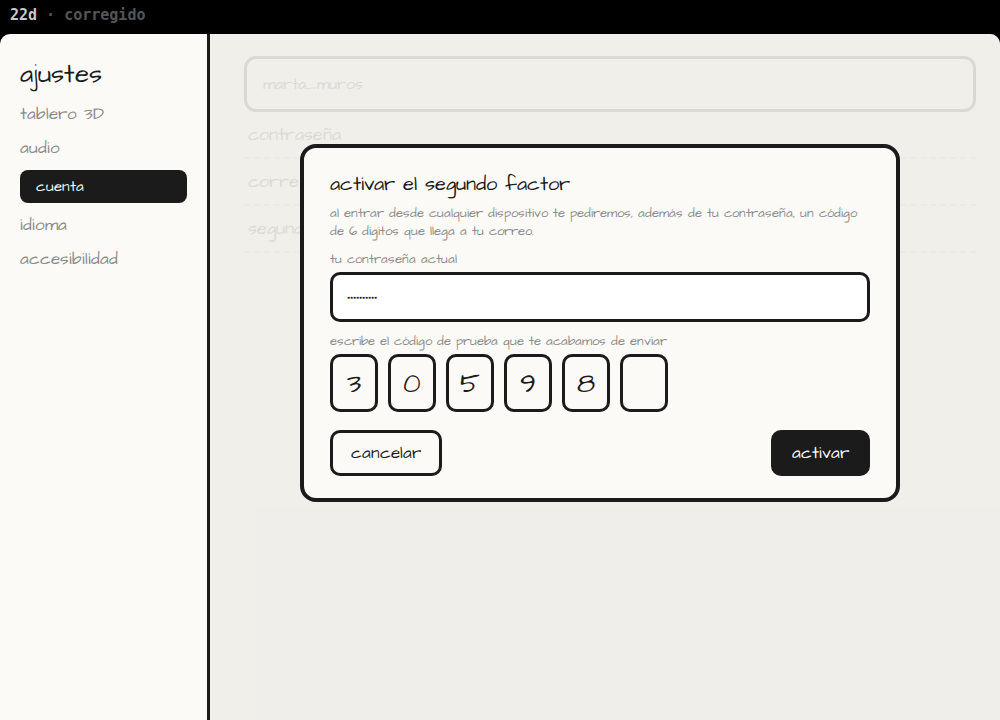
\includegraphics[width=\linewidth]{Prototipos/corregidos/22d}\par\smallskip
{\footnotesize\RaggedRight \textbf{22d corregido: Activar el segundo factor (nueva)}\par}
\end{minipage}
\par
\par\medskip\noindent
\begin{minipage}[t]{0.48\textwidth}
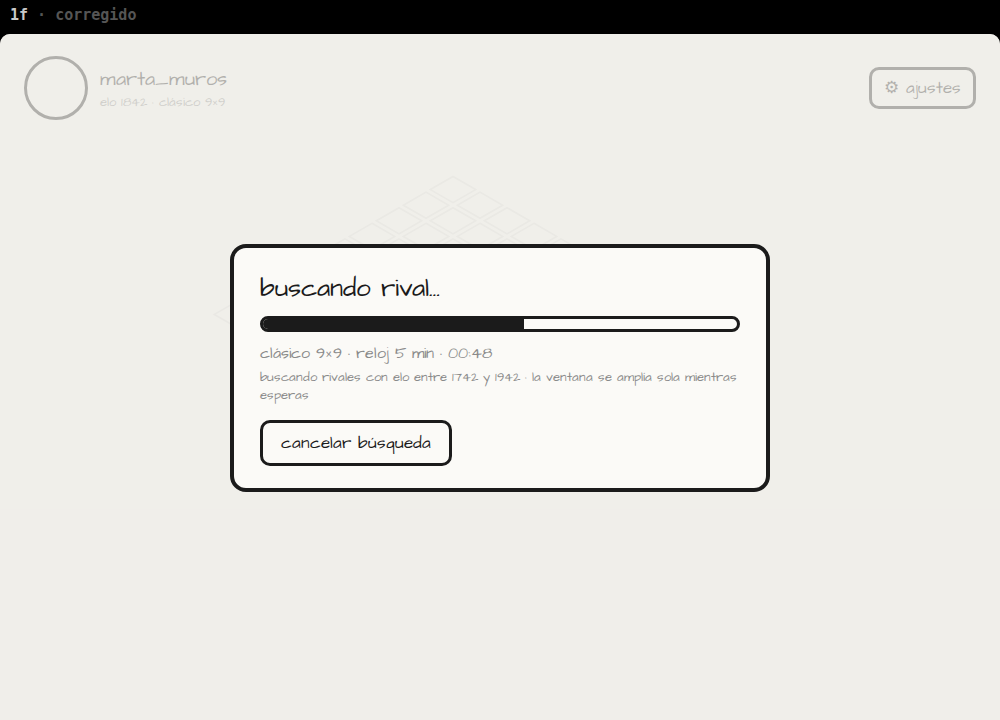
\includegraphics[width=\linewidth]{Prototipos/corregidos/1f}\par\smallskip
{\footnotesize\RaggedRight \textbf{1f corregido: Buscando rival}\par}
\end{minipage}\hfill
\begin{minipage}[t]{0.48\textwidth}
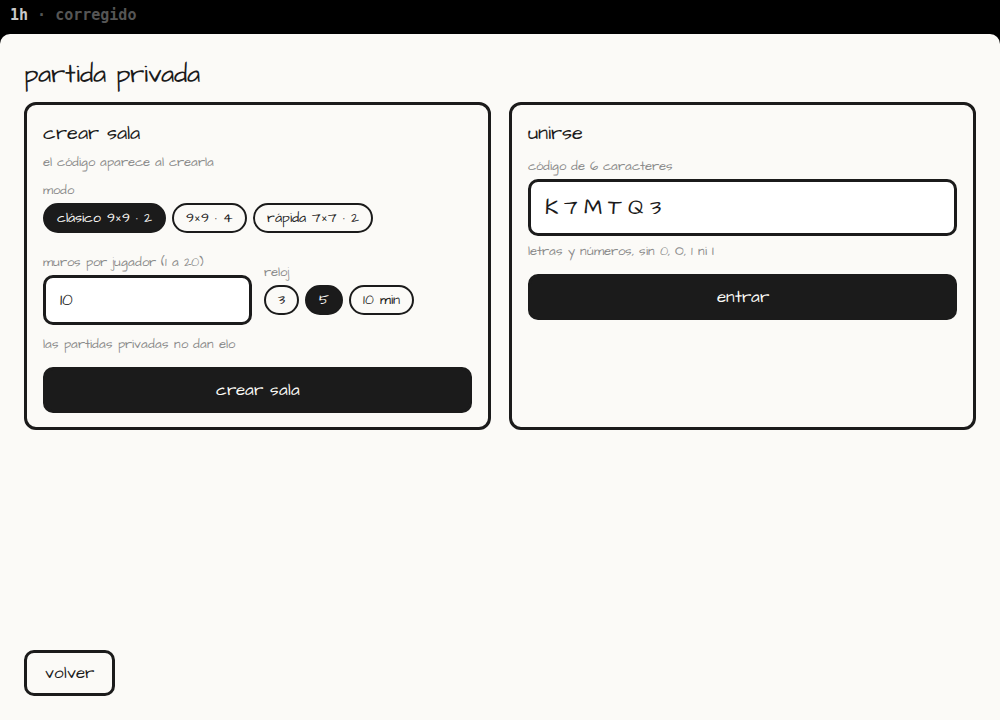
\includegraphics[width=\linewidth]{Prototipos/corregidos/1h}\par\smallskip
{\footnotesize\RaggedRight \textbf{1h corregido: Partida privada: crear o unirse}\par}
\end{minipage}
\par
\par\medskip\noindent
\begin{minipage}[t]{0.48\textwidth}
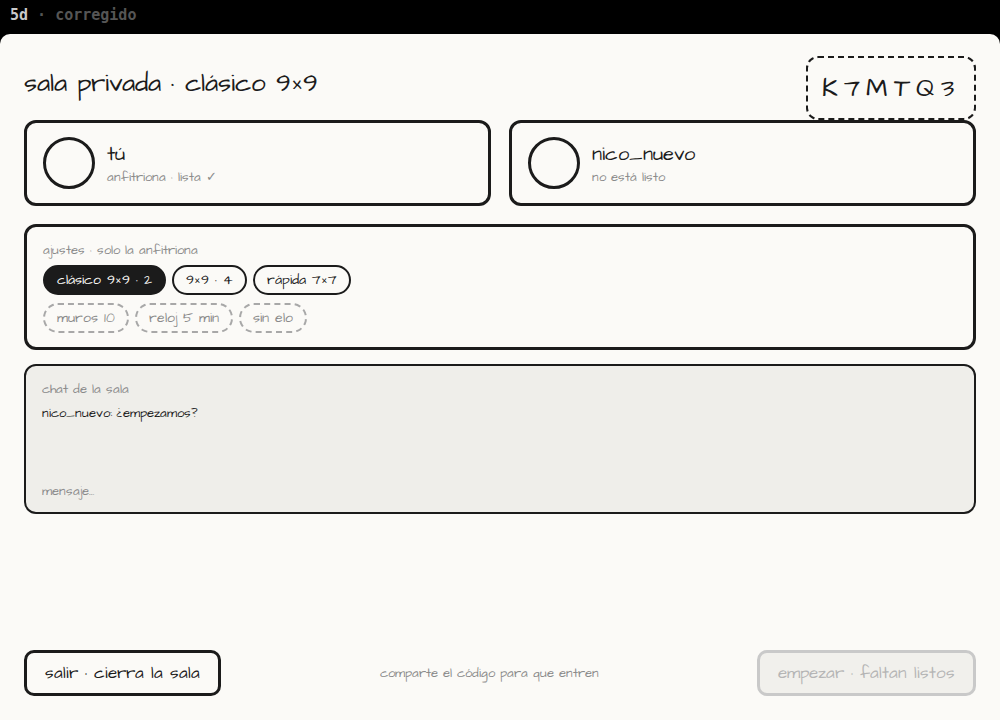
\includegraphics[width=\linewidth]{Prototipos/corregidos/5d}\par\smallskip
{\footnotesize\RaggedRight \textbf{5d corregido: Sala de espera, 2 jugadores}\par}
\end{minipage}\hfill
\begin{minipage}[t]{0.48\textwidth}
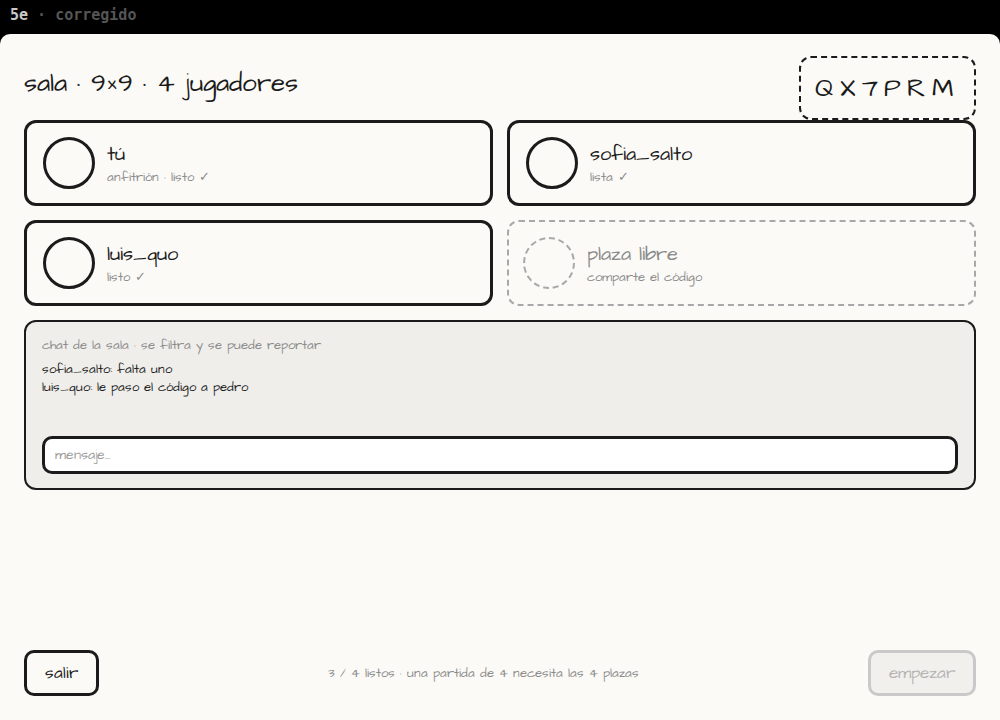
\includegraphics[width=\linewidth]{Prototipos/corregidos/5e}\par\smallskip
{\footnotesize\RaggedRight \textbf{5e corregido: Sala de espera, 4 plazas}\par}
\end{minipage}
\par
\par\medskip\noindent
\begin{minipage}[t]{0.48\textwidth}
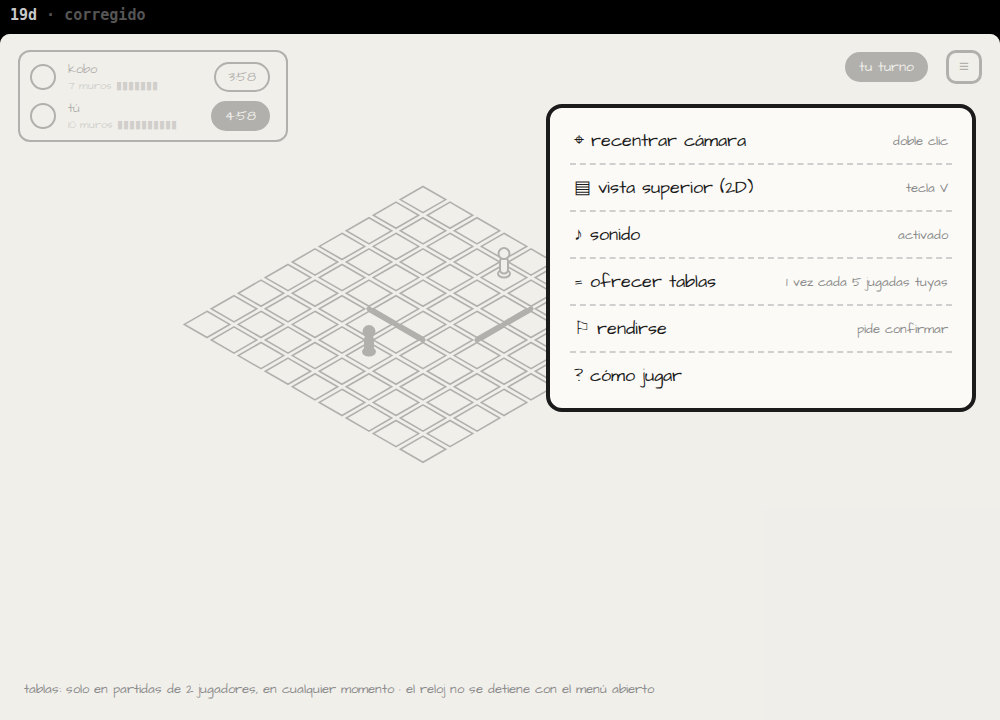
\includegraphics[width=\linewidth]{Prototipos/corregidos/19d}\par\smallskip
{\footnotesize\RaggedRight \textbf{19d corregido: Menú de partida}\par}
\end{minipage}\hfill
\begin{minipage}[t]{0.48\textwidth}
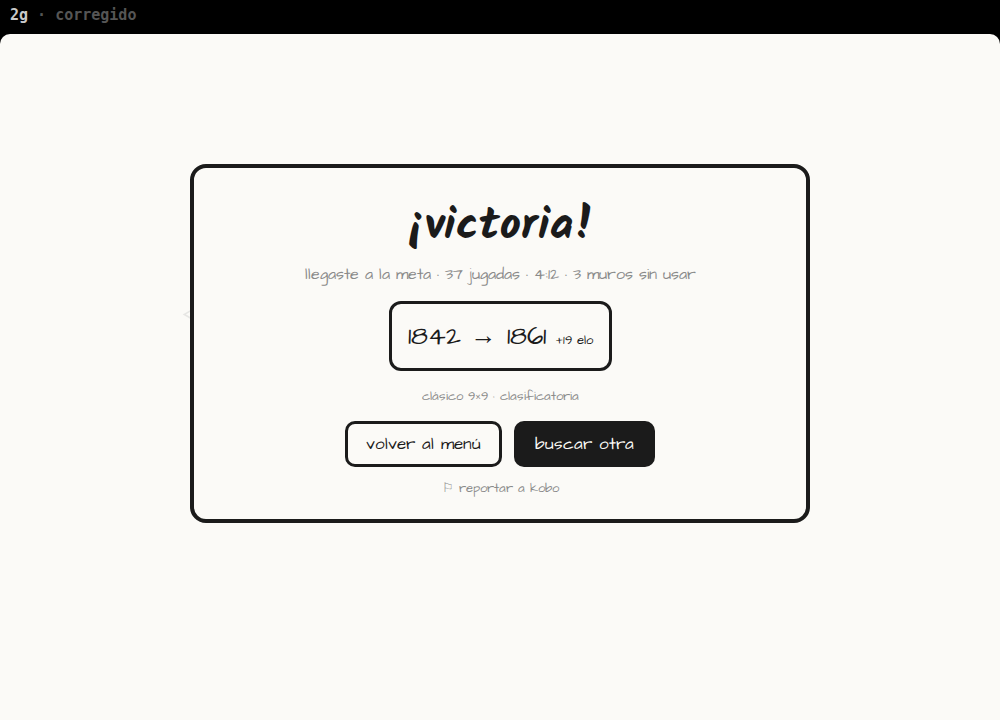
\includegraphics[width=\linewidth]{Prototipos/corregidos/2g}\par\smallskip
{\footnotesize\RaggedRight \textbf{2g corregido: Fin de partida}\par}
\end{minipage}
\par
\par\medskip\noindent
\begin{minipage}[t]{0.48\textwidth}
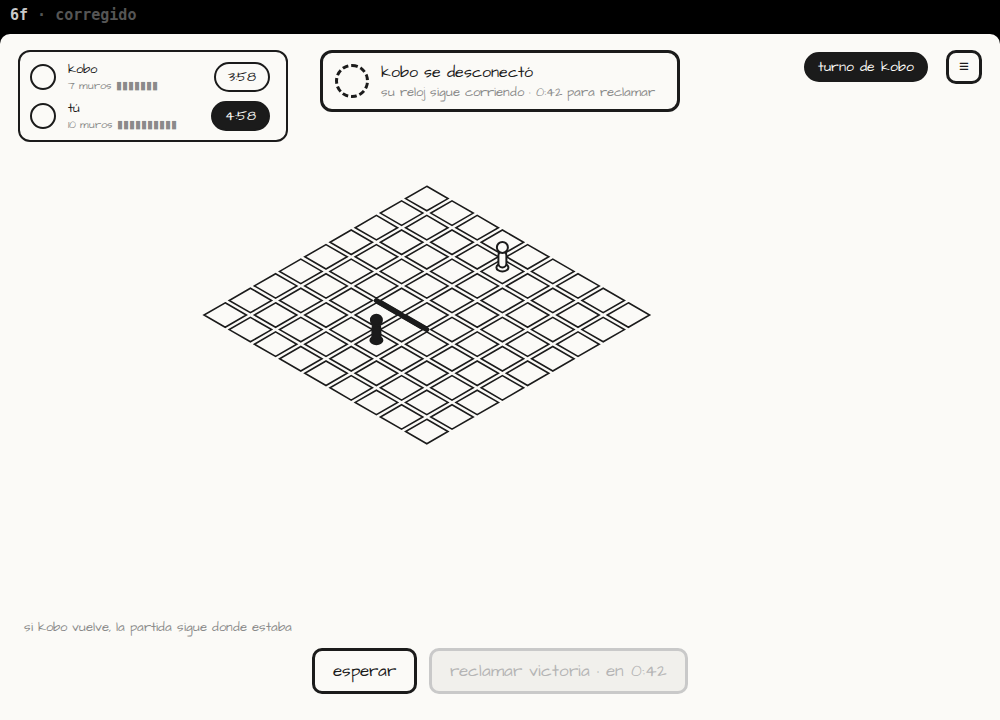
\includegraphics[width=\linewidth]{Prototipos/corregidos/6f}\par\smallskip
{\footnotesize\RaggedRight \textbf{6f corregido: Rival desconectado}\par}
\end{minipage}\hfill
\begin{minipage}[t]{0.48\textwidth}
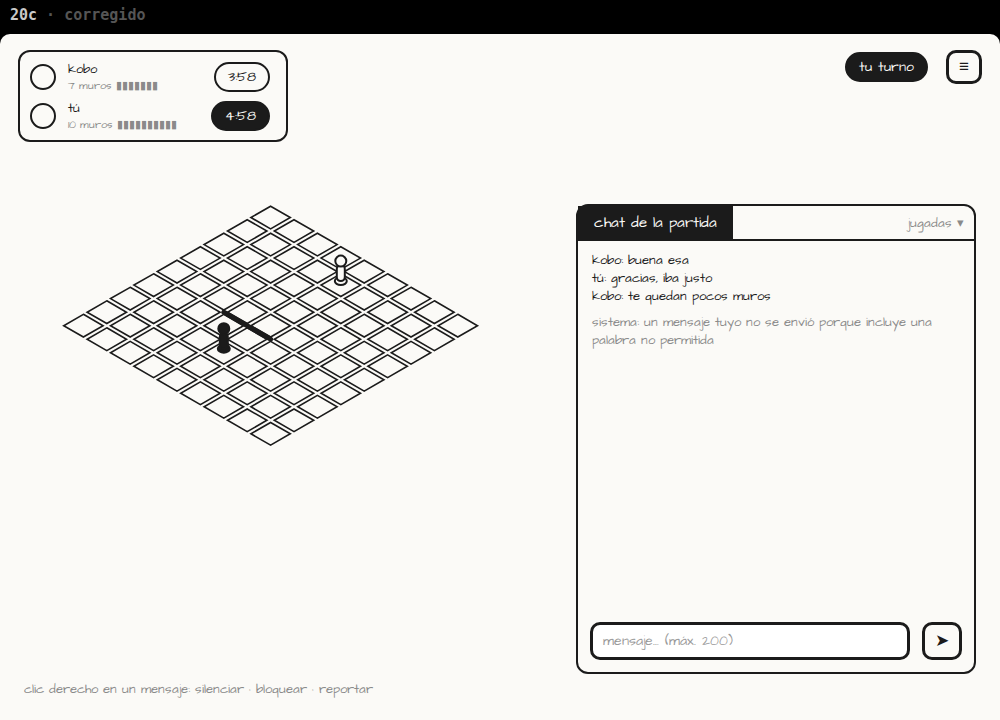
\includegraphics[width=\linewidth]{Prototipos/corregidos/20c}\par\smallskip
{\footnotesize\RaggedRight \textbf{20c corregido: Chat en partida}\par}
\end{minipage}
\par
\par\medskip\noindent
\begin{minipage}[t]{0.48\textwidth}
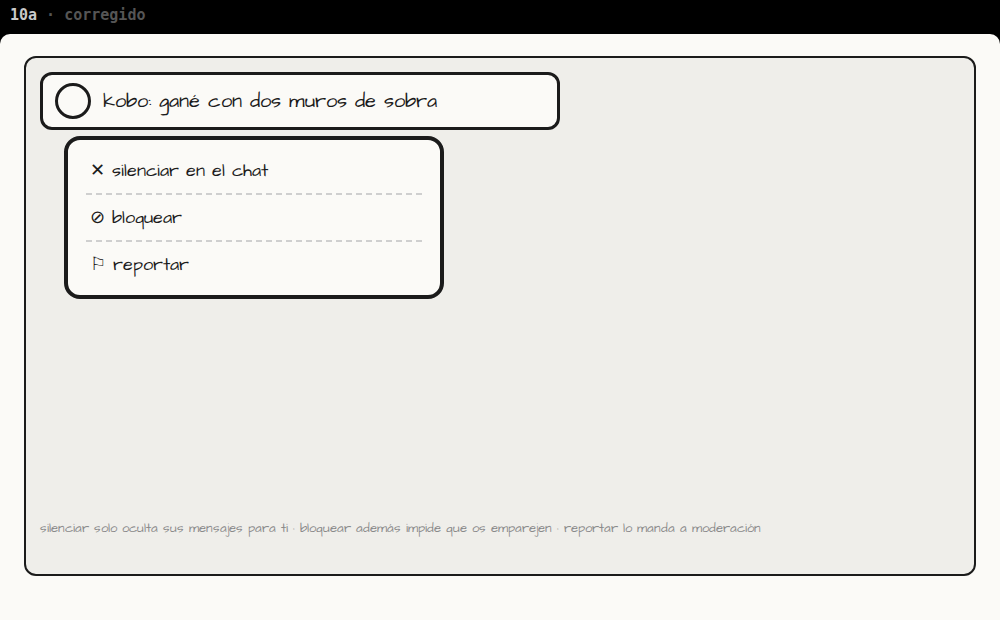
\includegraphics[width=\linewidth]{Prototipos/corregidos/10a}\par\smallskip
{\footnotesize\RaggedRight \textbf{10a corregido: Menú de un jugador}\par}
\end{minipage}\hfill
\begin{minipage}[t]{0.48\textwidth}
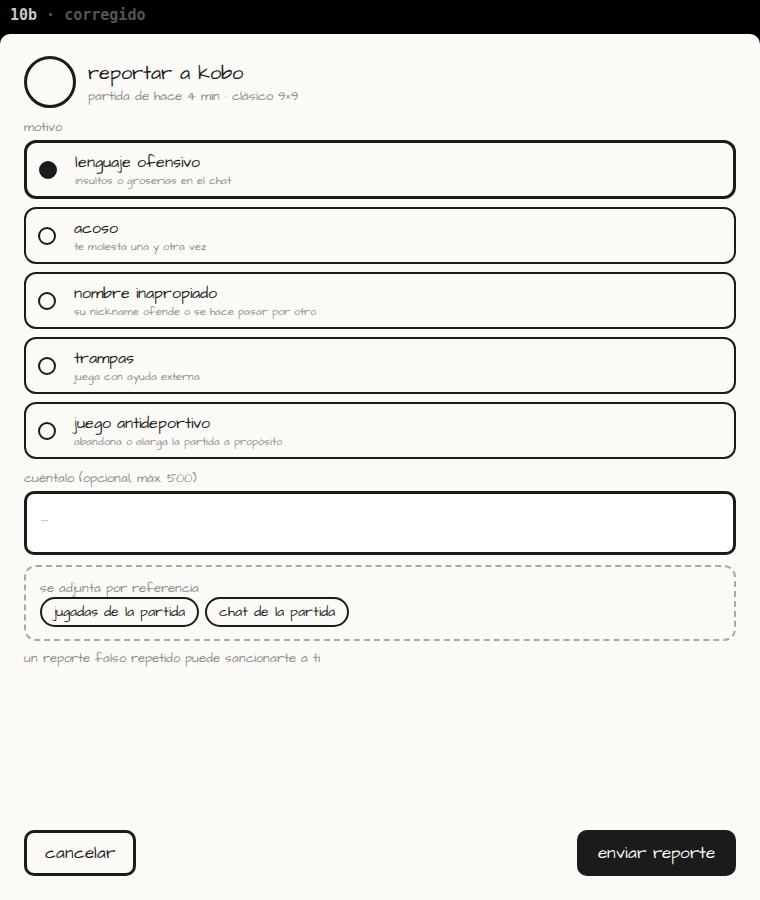
\includegraphics[width=\linewidth]{Prototipos/corregidos/10b}\par\smallskip
{\footnotesize\RaggedRight \textbf{10b corregido: Reportar}\par}
\end{minipage}
\par
\par\medskip\noindent
\begin{minipage}[t]{0.48\textwidth}
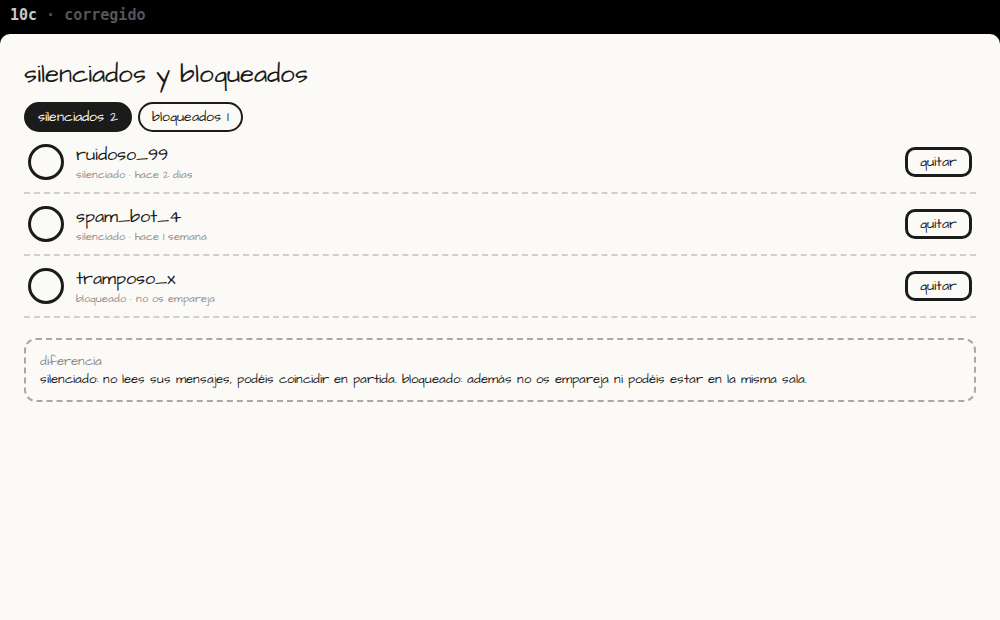
\includegraphics[width=\linewidth]{Prototipos/corregidos/10c}\par\smallskip
{\footnotesize\RaggedRight \textbf{10c corregido: Silenciados y bloqueados}\par}
\end{minipage}\hfill
\begin{minipage}[t]{0.48\textwidth}
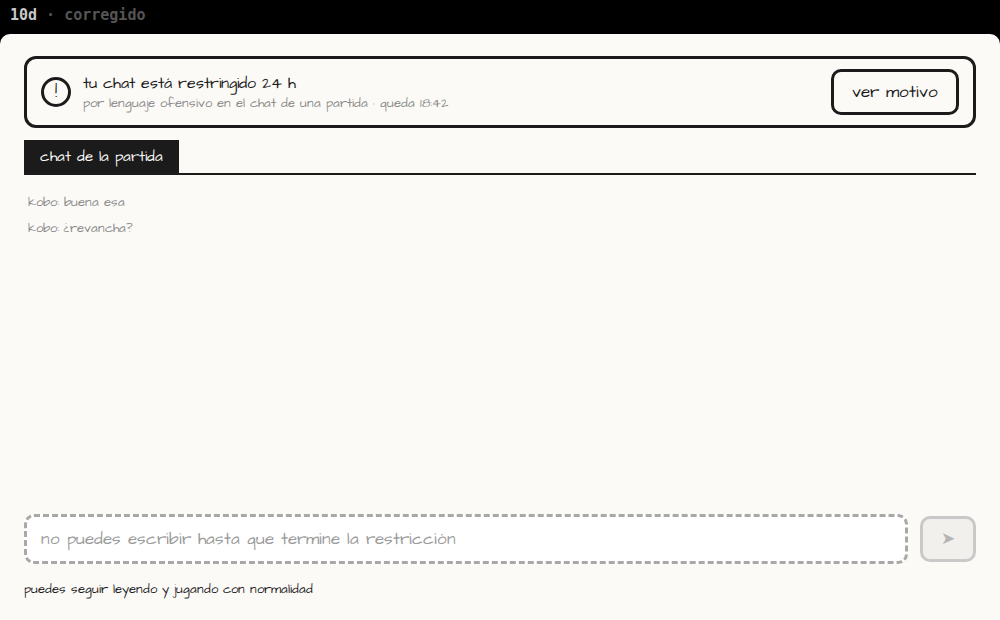
\includegraphics[width=\linewidth]{Prototipos/corregidos/10d}\par\smallskip
{\footnotesize\RaggedRight \textbf{10d corregido: Chat restringido}\par}
\end{minipage}
\par
\par\medskip\noindent
\begin{minipage}[t]{0.48\textwidth}
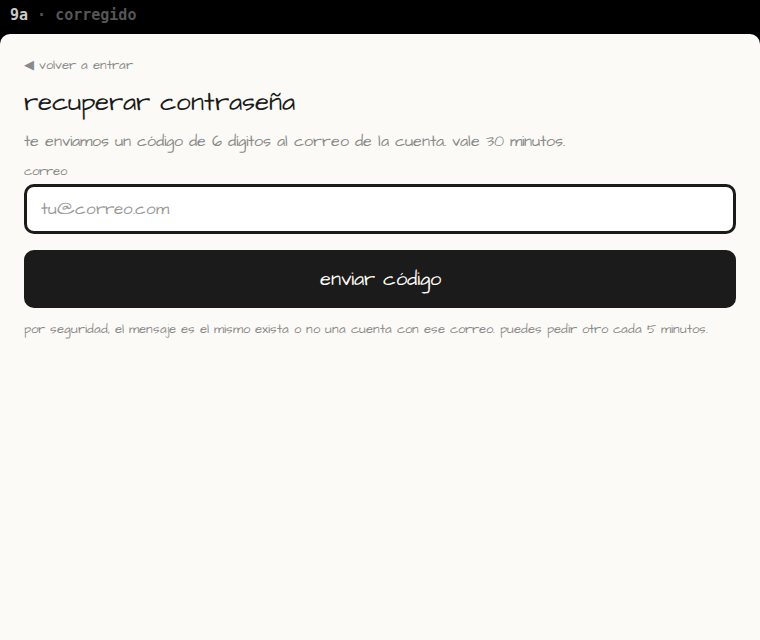
\includegraphics[width=\linewidth]{Prototipos/corregidos/9a}\par\smallskip
{\footnotesize\RaggedRight \textbf{9a corregido: Recuperar contraseña: pedir el código}\par}
\end{minipage}\hfill
\begin{minipage}[t]{0.48\textwidth}
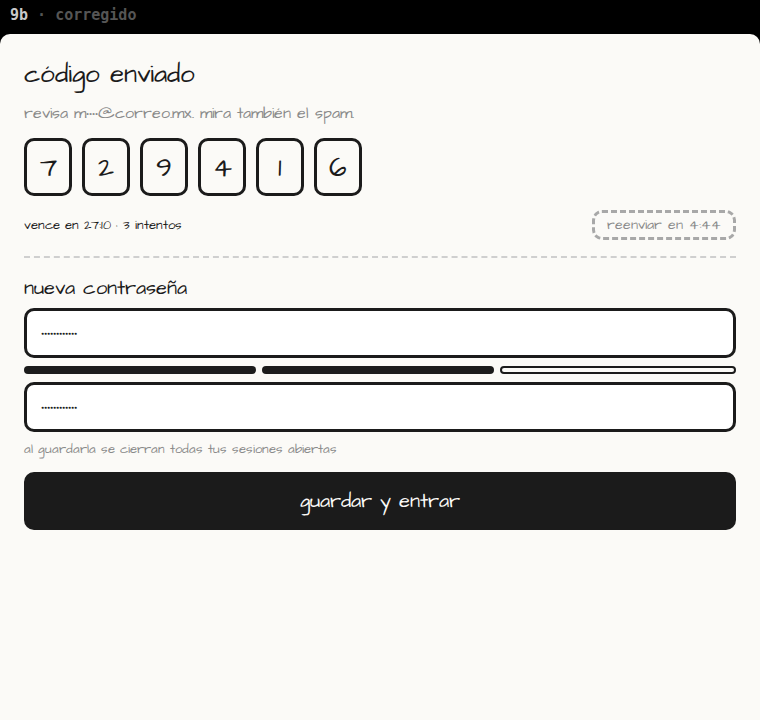
\includegraphics[width=\linewidth]{Prototipos/corregidos/9b}\par\smallskip
{\footnotesize\RaggedRight \textbf{9b corregido: Recuperar contraseña: código y nueva contraseña}\par}
\end{minipage}
\par
\par\medskip\noindent
\begin{minipage}[t]{0.48\textwidth}
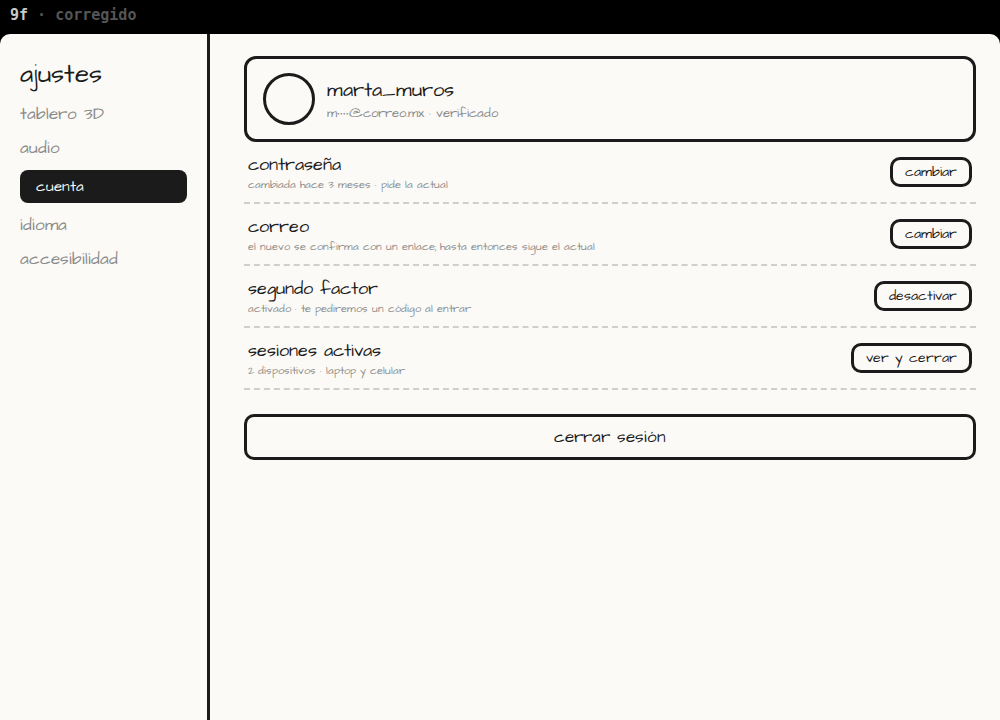
\includegraphics[width=\linewidth]{Prototipos/corregidos/9f}\par\smallskip
{\footnotesize\RaggedRight \textbf{9f corregido: Ajustes de cuenta}\par}
\end{minipage}\hfill
\begin{minipage}[t]{0.48\textwidth}
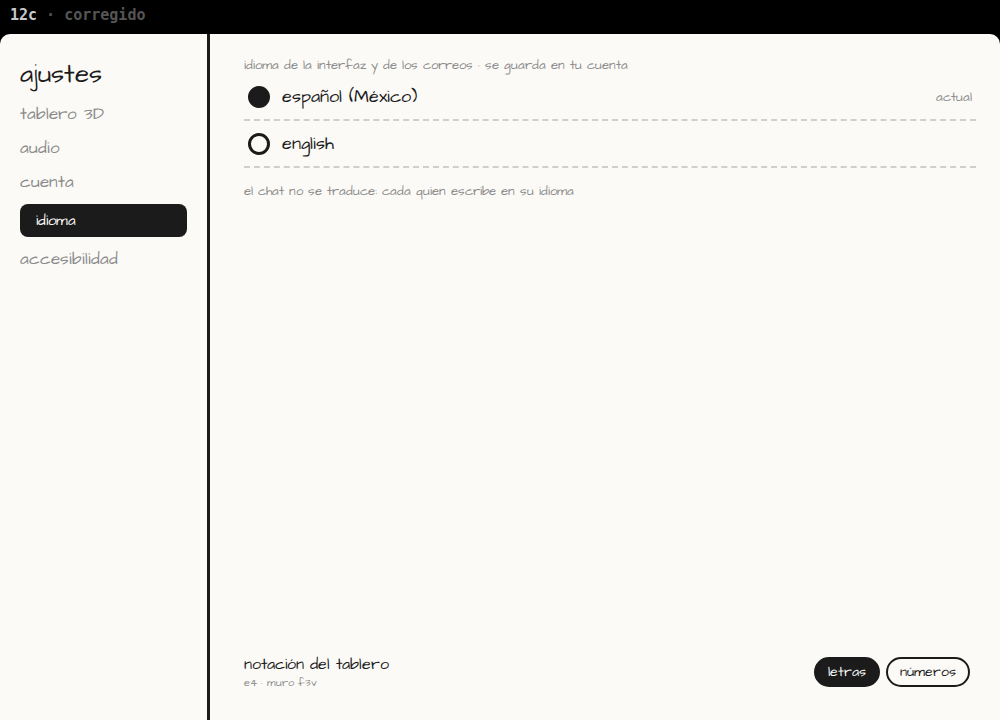
\includegraphics[width=\linewidth]{Prototipos/corregidos/12c}\par\smallskip
{\footnotesize\RaggedRight \textbf{12c corregido: Ajustes: idioma}\par}
\end{minipage}
\par
\par\medskip\noindent
\begin{minipage}[t]{0.48\textwidth}
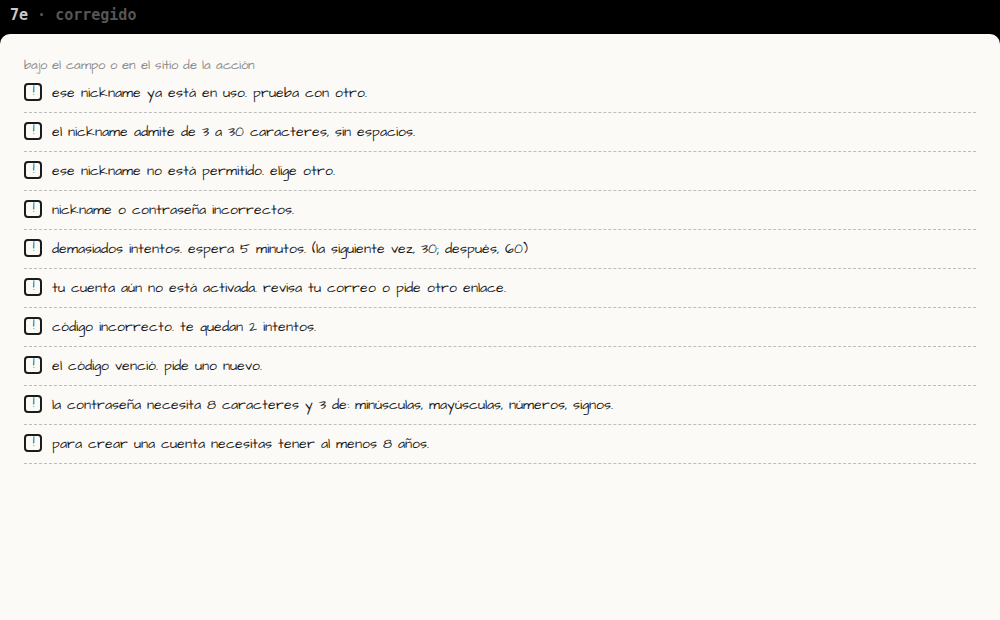
\includegraphics[width=\linewidth]{Prototipos/corregidos/7e}\par\smallskip
{\footnotesize\RaggedRight \textbf{7e corregido: Errores de cuenta}\par}
\end{minipage}\hfill
\begin{minipage}[t]{0.48\textwidth}
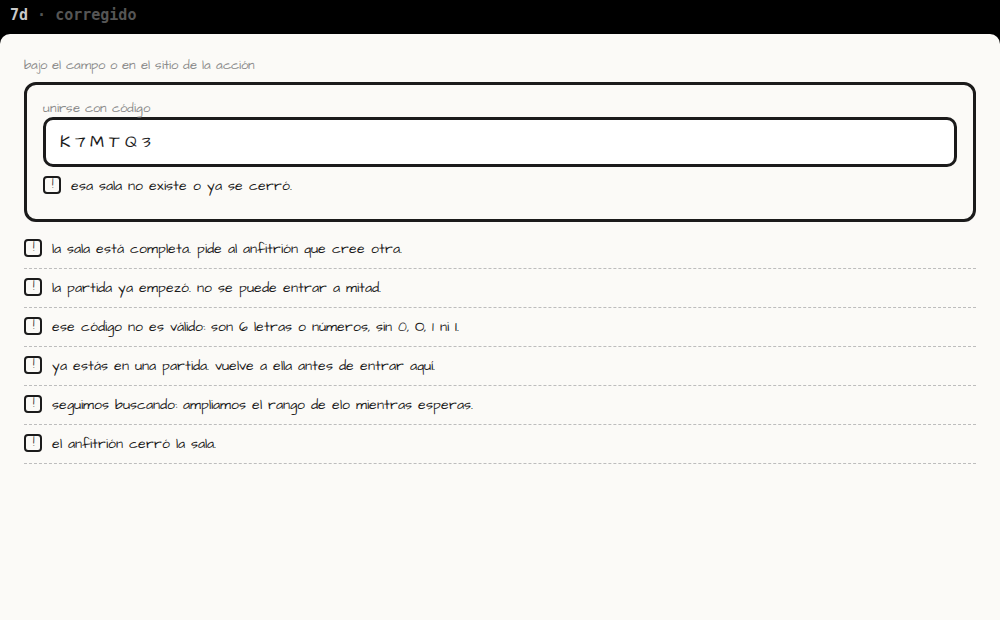
\includegraphics[width=\linewidth]{Prototipos/corregidos/7d}\par\smallskip
{\footnotesize\RaggedRight \textbf{7d corregido: Errores de salas y emparejamiento}\par}
\end{minipage}
\par
\par\medskip\noindent
\begin{minipage}[t]{0.48\textwidth}
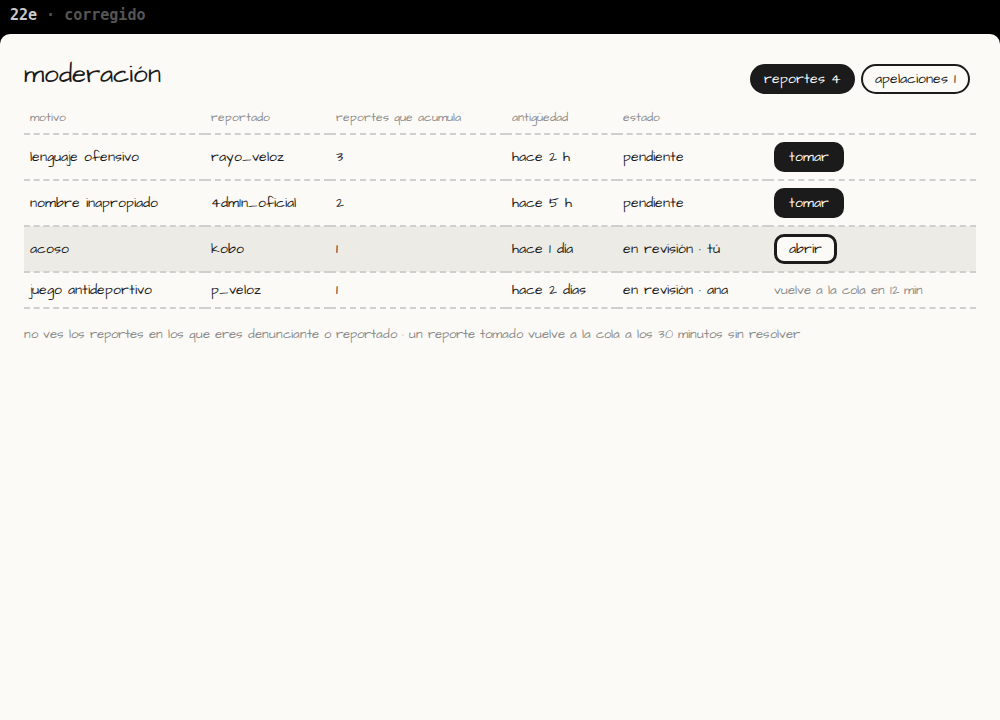
\includegraphics[width=\linewidth]{Prototipos/corregidos/22e}\par\smallskip
{\footnotesize\RaggedRight \textbf{22e corregido: Cola de moderación (nueva)}\par}
\end{minipage}\hfill
\begin{minipage}[t]{0.48\textwidth}
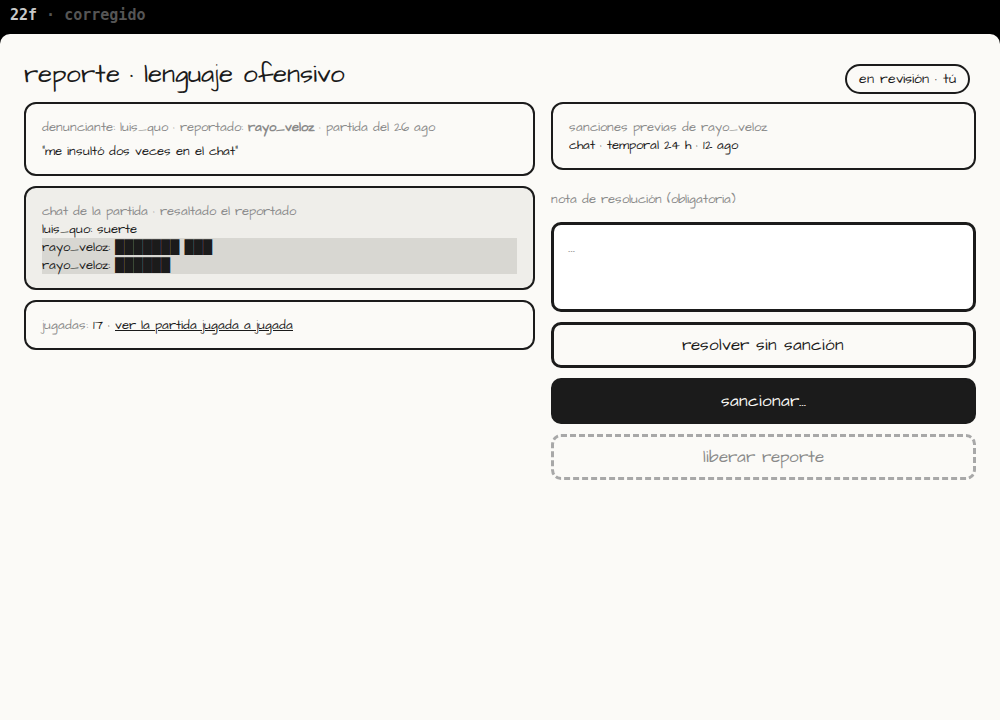
\includegraphics[width=\linewidth]{Prototipos/corregidos/22f}\par\smallskip
{\footnotesize\RaggedRight \textbf{22f corregido: Revisar un reporte (nueva)}\par}
\end{minipage}
\par
\par\medskip\noindent
\begin{minipage}[t]{0.48\textwidth}
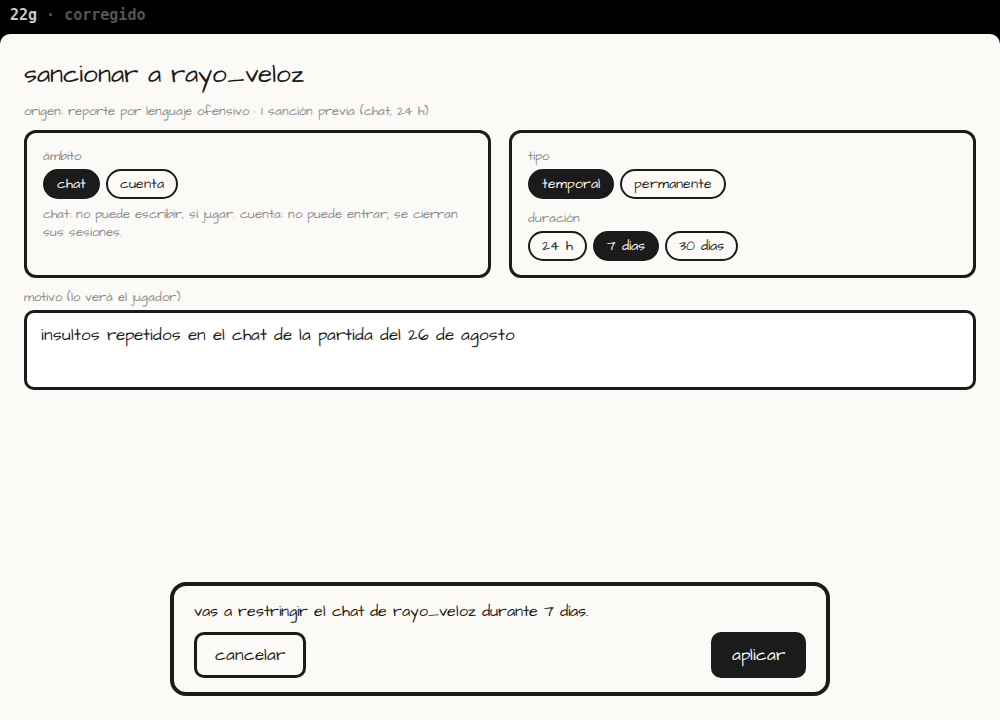
\includegraphics[width=\linewidth]{Prototipos/corregidos/22g}\par\smallskip
{\footnotesize\RaggedRight \textbf{22g corregido: Aplicar una sanción (nueva)}\par}
\end{minipage}\hfill
\begin{minipage}[t]{0.48\textwidth}
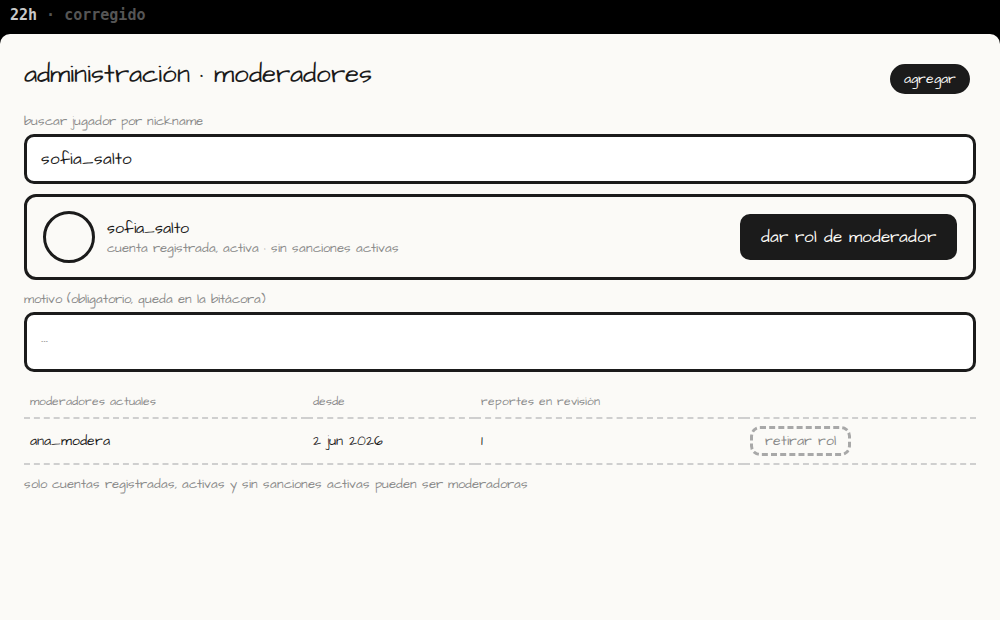
\includegraphics[width=\linewidth]{Prototipos/corregidos/22h}\par\smallskip
{\footnotesize\RaggedRight \textbf{22h corregido: Agregar un moderador (nueva)}\par}
\end{minipage}
\par

\par
